% !Mode:: "TeX:UTF-8" 

\BiSection{2.7}{Figures}

\fancyhead[R]{本题2.7由QC.Z完成}

解:

\scalebox{3}{(a)}

当$V_{out}<1V$时,NFET源漏交换

		\begin{figure}[H] %H为当前位置,!htb为忽略美学标准,htbp为浮动图形
	\begin{minipage}{\linewidth}
		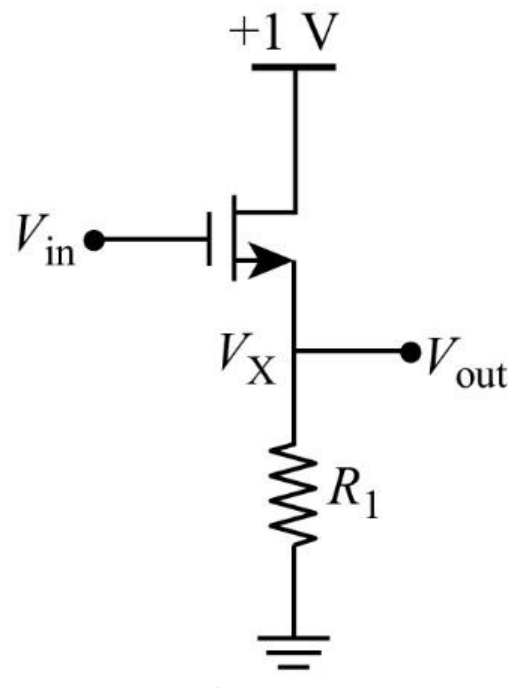
\includegraphics{2.7-1}
	\end{minipage}
	\caption*{图1} %最终文档中希望显示的图片标题
\end{figure}

当$V_{TH}>V_{in}>0$即$0.7V>V_{in}>0$时,NFET关

当NFET在饱和区时,$V_{G}-V_{TH}<V_{D}$;所以当$0.7V<V_{in}<1.7V$时,NFET在饱和区

$I_D=\frac{1}{2}\mu_nC_{ox}\frac{W}{L}(V_{GS}-V_{TH})^2=\frac{1}{2}\mu_nC_{ox}\frac{W}{L}(V_{in}-V_{out}-0.7)^2$

由欧姆定律得$I_D=\frac{V_{out}}{R_1}$

联立以上二式得$\frac{V_{out}}{R_1}=\frac{1}{2}\mu_nC_{ox}\frac{W}{L}(V_{in}-V_{out}-0.7)^2$

当$3V>V_{in}>1.7V$时,NFET在线性区

$I_D=\mu_nC_{ox}\frac{W}{L}[(V_{GS}-V_{TH})V_{DS}-\frac{1}{2}V_{DS}^2]=\mu_nC_{ox}\frac{W}{L}[(V_{in}-V_{out}-0.7)(1-V_{out})-\frac{1}{2}(1-V_{out})^2]$

		\begin{figure}[H] %H为当前位置,!htb为忽略美学标准,htbp为浮动图形
	\begin{minipage}{\linewidth}
		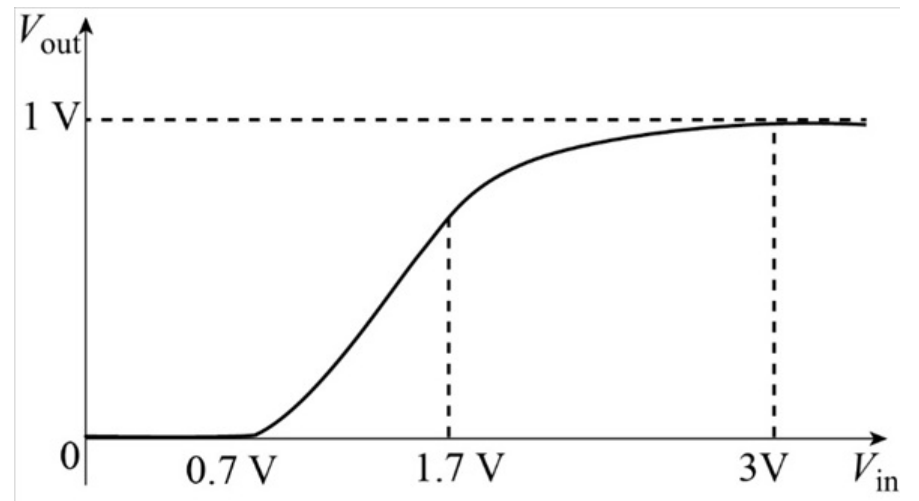
\includegraphics{2.7-2}
	\end{minipage}
	\caption*{图2} %最终文档中希望显示的图片标题
\end{figure}

\scalebox{3}{(b)}

因为$V_{out}<V_{in}$时,所以NFET源漏交换

		\begin{figure}[H] %H为当前位置,!htb为忽略美学标准,htbp为浮动图形
	\begin{minipage}{\linewidth}
		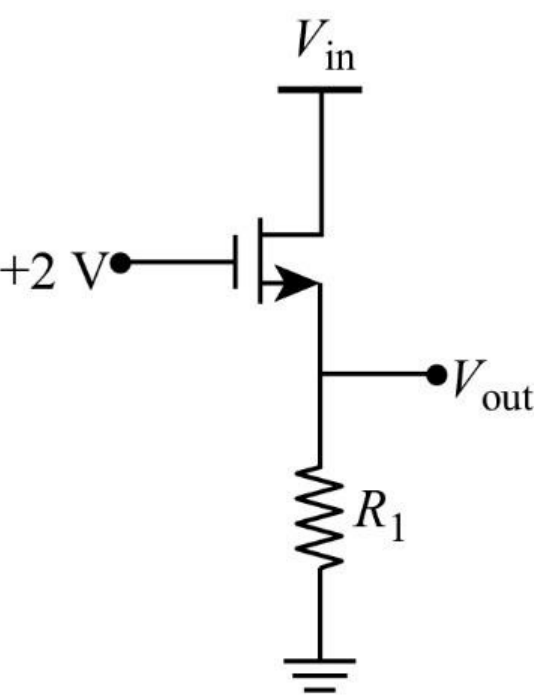
\includegraphics{2.7-3}
	\end{minipage}
	\caption*{图3} %最终文档中希望显示的图片标题
\end{figure}

当$V_{G}-V_{TH}>V_{D}$即$1.3V>V_{in}>0V$时,NFET在线性区

$I_D=\mu_nC_{ox}\frac{W}{L}[(V_{GS}-V_{TH})V_{DS}-\frac{1}{2}V_{DS}^2]=\mu_nC_{ox}\frac{W}{L}[(2-V_{out}-0.7)(V_{in}-V_{out})-\frac{1}{2}(V_{in}-V_{out})^2]$

由欧姆定律得$I_D=\frac{V_{out}}{R_1}$

联立以上二式得$\frac{V_{out}}{R_1}=\mu_nC_{ox}\frac{W}{L}[(2-V_{out}-0.7)(V_{in}-V_{out})-\frac{1}{2}(V_{in}-V_{out})^2]$

当$3V>V_{in}>1.3V$时,NFET在饱和区

$I_D=\frac{1}{2}\mu_nC_{ox}\frac{W}{L}(V_{GS}-V_{TH})^2=\frac{1}{2}\mu_nC_{ox}\frac{W}{L}(2-V_{out}-0.7)^2$

$\frac{V_{out}}{R_1}=\frac{1}{2}\mu_nC_{ox}\frac{W}{L}(2-V_{out}-0.7)^2$

		\begin{figure}[H] %H为当前位置,!htb为忽略美学标准,htbp为浮动图形
	\begin{minipage}{\linewidth}
		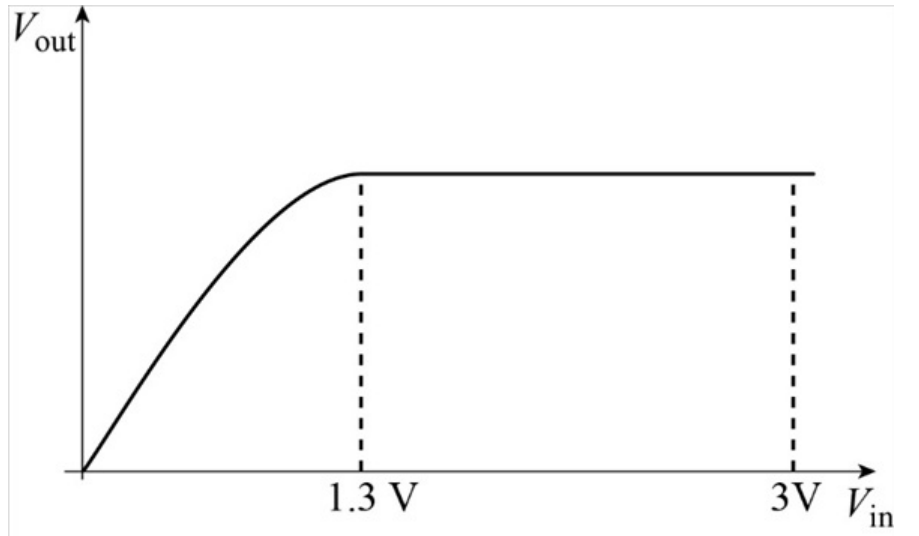
\includegraphics{2.7-4}
	\end{minipage}
	\caption*{图4} %最终文档中希望显示的图片标题
\end{figure}

\scalebox{3}{(c)}

当$V_{G}-V_{TH}>V_{D}$即$2.3V>V_{in}>0V$时,NFET在线性区

$I_D=\mu_nC_{ox}\frac{W}{L}[(V_{GS}-V_{TH})V_{DS}-\frac{1}{2}V_{DS}^2]=\mu_nC_{ox}\frac{W}{L}[(3-V_{out}-0.7)(V_{in}-V_{out})-\frac{1}{2}(V_{in}-V_{out})^2]$

由欧姆定律得$I_D=\frac{V_{out}}{R_1}$

联立以上二式得$\frac{V_{out}}{R_1}=\mu_nC_{ox}\frac{W}{L}[(3-V_{out}-0.7)(V_{in}-V_{out})-\frac{1}{2}(V_{in}-V_{out})^2]$

当$3V>V_{in}>2.3V$时,NFET在饱和区

$I_D=\frac{1}{2}\mu_nC_{ox}\frac{W}{L}(V_{GS}-V_{TH})^2=\frac{1}{2}\mu_nC_{ox}\frac{W}{L}(3-V_{out}-0.7)^2$

$\frac{V_{out}}{R_1}=\frac{1}{2}\mu_nC_{ox}\frac{W}{L}(3-V_{out}-0.7)^2$

\begin{figure}[H] %H为当前位置,!htb为忽略美学标准,htbp为浮动图形
	\begin{minipage}{\linewidth}
		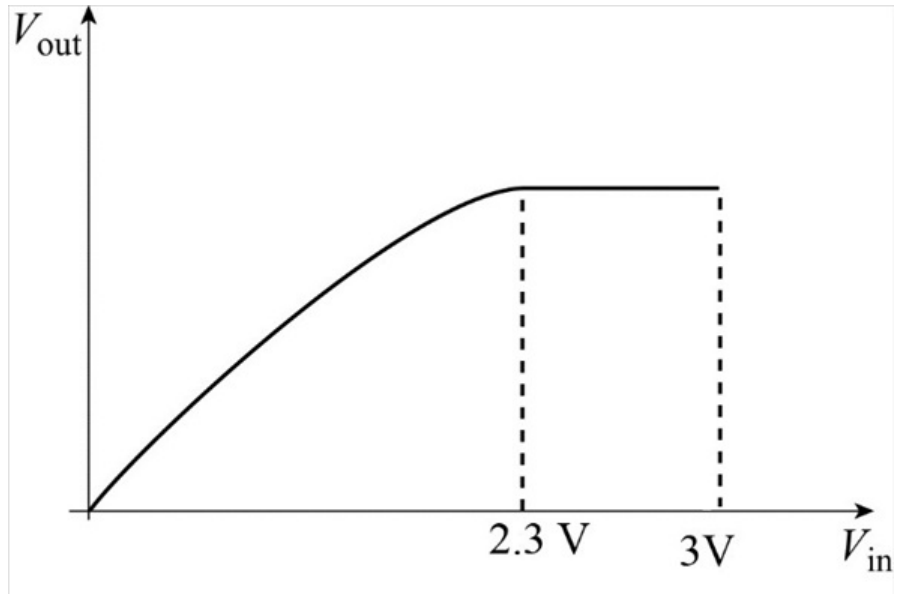
\includegraphics{2.7-5}
	\end{minipage}
	\caption*{图5} %最终文档中希望显示的图片标题
\end{figure}

\scalebox{3}{(d)}

当$V_{SG}<|V_{TH}|$即$1.8V>V_{in}>0V$时,PFET关

当$V_{G}+|V_{TH}|>V_{D}$即$1.8V>V_{out}$且$1.8V<V_{in}$时,PFET在饱和区。\textcolor{blue}{(由电路图得源极总是大于漏极,PFET电压低的为漏极,下面求PFET在饱和区时$V_{in}$的范围)}

$I_D=\frac{1}{2}\mu_pC_{ox}\frac{W}{L}(V_{in}-1.8V)^2$

$\frac{V_{out}}{R_1}=\frac{1}{2}\mu_pC_{ox}\frac{W}{L}(V_{in}-1.8V)^2$

$V_{out}=\frac{1}{2}\mu_pC_{ox}{R_1}\frac{W}{L}(V_{in}-1.8V)^2$\ding{172}

$1.8V=\frac{1}{2}\mu_pC_{ox}{R_1}\frac{W}{L}(V_{in}-1.8V)^2$

\begin{figure}[H] %H为当前位置,!htb为忽略美学标准,htbp为浮动图形
	\begin{minipage}{\linewidth}
		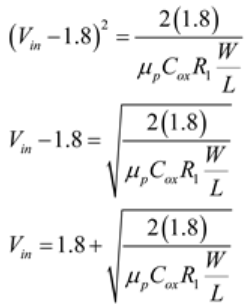
\includegraphics{2.7-6}
	\end{minipage}
\end{figure}

当$1.8V>V_{out}$且$1.8V<V_{in}<1.8V+\sqrt{\frac{2(1.8V)}{\mu_pC_{ox}{R_1}\frac{W}{L}}}$时,PFET在饱和区

当$1.8V<V_{out}$且$V_{in}>1.8V+\sqrt{\frac{2(1.8V)}{\mu_pC_{ox}{R_1}\frac{W}{L}}}$时,PFET在线性区

$I_D=\mu_pC_{ox}\frac{W}{L}[(V_{in}-1.8V)(V_{in}-V_{out})-\frac{1}{2}(V_{in}-V_{out})^2]$

$\frac{V_{out}}{R_1}=\mu_pC_{ox}\frac{W}{L}[(V_{in}-1.8V)(V_{in}-V_{out})-\frac{1}{2}(V_{in}-V_{out})^2]$\ding{173}

















\begin{figure}[H] %H为当前位置,!htb为忽略美学标准,htbp为浮动图形
	\begin{minipage}{\linewidth}
		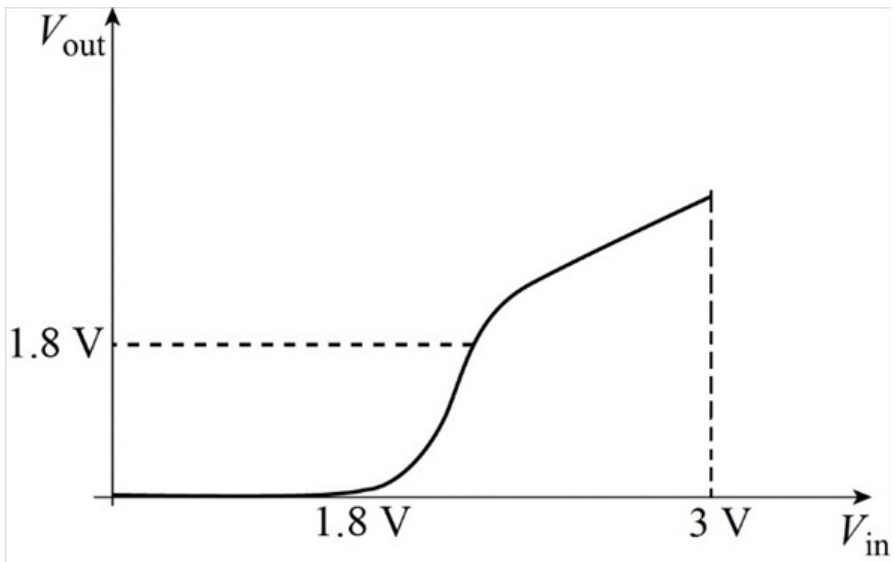
\includegraphics{2.7-7}
	\end{minipage}
	\caption*{图6} %最终文档中希望显示的图片标题
\end{figure}














